%\listfiles

%% Tipo de documento e a classe a ser usada para sua formatação.
\documentclass[tese]{UFRuralRJ}

%% Um tipo específico de monografia pode ser informado como parâmetro opcional:
%\documentclass[tese]{UFRuralRJ}

%% A opção 'openright' força inícios de capítulos em páginas ímpares
%\documentclass[openright]{UFRuralRJ}

%% Use a opção 'twoside' para gerar uma versão frente-e-verso
%\documentclass[twoside]{UFRuralRJ}

%%==============================================================================
%% Pacotes - língua, codificação e fonte
%%==============================================================================

\usepackage[brazilian]{babel} %% use 'english' ao invés de 'brazilian' para documento escrito em inglês
\usepackage[T1]{fontenc} %% Conjunto de caracteres correto
%\usepackage{times} %% Usar fonte Adobe Times Roman, equivalente à Times New Roman
\usepackage[utf8]{inputenc} %% Para acentuação correta

%%==============================================================================
%% Pacotes - formatação de equações e números
%%==============================================================================

\usepackage{amsmath,latexsym,amssymb}
\usepackage{siunitx}                  %% Sistema Internacional de Unidades

%%==============================================================================
%% Pacotes - formatação de figuras
%%==============================================================================

%% Importar figuras corretamente
\usepackage{graphicx}

%% Diretório onde estão as figuras dos capítulos
\graphicspath{{capitulos-b/figuras/}}

\usepackage{float}
\usepackage{wrapfig}

%%==============================================================================
%% Pacotes - formatação de hyperlinks
%%==============================================================================
%% Opção 'hidelinks' disponível no pacote 'hyperref' a partir da versão 
%% 2011-02-05  6.82a. 'hidelinks' retira os retângulos do entorno das palavras
%% com links.

\usepackage[%hidelinks%, 
            bookmarksopen=true,linktoc=none,colorlinks=true,
            linkcolor=blue,citecolor=blue,filecolor=magenta,urlcolor=blue,
            pdftitle={Este título é muito legal para uma tese escrita em português},
            pdfauthor={Nome do Melhor Estudante da Rural},
            pdfsubject={Tese de Doutorado},
            pdfkeywords={LaTeX, UFRuralRJ, Documentos acadêmicos}
            ]{hyperref}

%% Definição das margens
\usepackage[inner = 30mm, outer = 20mm, top = 30mm, bottom = 20mm]{geometry}

%% Se o pacote 'hyperref' acima foi carregado, a linha abaixo corrige um bug na 
%% hora de montar o sumário da lista de figuras e tabelas. Comente a linha se o
%% pacote 'hyperref' não foi carregado.

%%=============================================================================
%% Trampa para corrigir o bug do hyperref que redefine o caption das figuras e das
%% tabelas, n�o colocando o nome ``Figura'' antes do n�mero do mesmo na lista
%%=============================================================================

\makeatletter

\long\def\@caption#1[#2]#3{%
  \expandafter\ifx\csname if@capstart\expandafter\endcsname
                  \csname iftrue\endcsname
    \global\let\@currentHref\hc@currentHref
  \else
    \hyper@makecurrent{\@captype}%
  \fi
  \@ifundefined{NR@gettitle}{%
    \def\@currentlabelname{#2}%
  }{%
    \NR@gettitle{#2}%
  }%
  \par\addcontentsline{\csname ext@#1\endcsname}{#1}{%
    \protect\numberline{\csname fnum@#1\endcsname ~-- }{\ignorespaces #2}%
  }%
  \begingroup
    \@parboxrestore
    \if@minipage
      \@setminipage
    \fi
    \normalsize
    \expandafter\ifx\csname if@capstart\expandafter\endcsname
                    \csname iftrue\endcsname
      \global\@capstartfalse
      \@makecaption{\csname fnum@#1\endcsname}{\ignorespaces#3}%
    \else
      \@makecaption{\csname fnum@#1\endcsname}{%
        \ignorespaces
        \ifHy@nesting
          \expandafter\hyper@@anchor\expandafter{\@currentHref}{#3}%
        \else
          \Hy@raisedlink{%
            \expandafter\hyper@@anchor\expandafter{%
              \@currentHref
            }{\relax}%
          }%
          #3%
        \fi
      }%
    \fi
    \par
  \endgroup
}

\makeatother

%%==============================================================================
%% Pacotes - formatação de verbatim
%%==============================================================================
%% O ambiente verbatim é o ambiente onde são inseridos exemplos de código fonte.
%% Está opção adiciona cor de fundo ao ambiente verbatim.
%% Comente para desabilitar.

\let\oldv\verbatim
\let\oldendv\endverbatim
\def\verbatim{\par\setbox0\vbox\bgroup\oldv}
\def\endverbatim{\oldendv\egroup\fboxsep0pt 
                 \noindent\colorbox[gray]{0.8}{\usebox0}\par}

%%==============================================================================
%% Pacotes - outros
%%==============================================================================

\usepackage{blindtext} %% Amostra de texto (\blindtext[1])

%%==============================================================================
%% Identificação do trabalho
%%==============================================================================
\titulo{Este título é muito legal para uma tese escrita em português} %% Título
\author{Rural}{Nome da Melhor Estudante da} %% Autor: sobrenome, nome
\autoratrue %% Usar no caso de uma AUTORA
\instituto{Instituto da Rural} %% Instituto
\curso{Curso de Pós-Graduação da Rural} %% Curso de pós-graduação
\area{Ciências} %% Área de concentração
\grau{Doutor em Ciências} %% Grau obtido
\nivel{Doutorado em Ciências} %% Nível do curso de pós-graduação
\local{Serop\'edica}{RJ}{Brasil} %% Local da defesa

%%==============================================================================
%% Identificação dos orientadores
%%==============================================================================
\advisor[Professor]{Dr.}{Rural}{Melhor Orientador da}{UFRRJ} %% Orientador
%\orientadoratrue %% Usar no caso de uma ORIENTADORA
\coadvisor[Pesquisador]{Dr.}{Rural}{Melhor Co-orientador da} %% Co-orientador
\coadvisor[Professora]{Dra.}{Rural}{Melhor Co-orientadora da} %% Co-orientadora
\coorientadorestrue %% Usar no caso de dois ou mais co-orientadores(as)

%%==============================================================================
%% Informações sobre a defesa
%%==============================================================================
\committee[Dr.]{Banca}{Melhor Presidente da}{UFRRJ} %% Presidente
\committee[Dra.]{Banca}{Melhor Integrante da}{UFRRJ} %% Examinador
\committee[Dr.]{Banca}{Melhor Integrante da}{UFRRJ} %% Examinador
\committee[Dra.]{Banca}{Outra Melhor Integrante da}{MEFR} %% Examinador
\committee[Dr.]{Banca}{Outro Melhor Integrante da}{MEFR} %% Examinador
\date{30}{Fevereiro}{2016} %% Data da defesa

%%==============================================================================
%% Início do documento
%%==============================================================================
\begin{document}

%%==============================================================================
%% Capa e folha de rosto
%%==============================================================================
\maketitle

%%=============================================================================
% Folha de aprovação
%%=============================================================================
\makeapprove

%%=============================================================================
%% Dedicatória (opcional)
%%=============================================================================
\clearpage\mbox{}\vfill\hspace{80mm}
\begin{minipage}{76mm}
  \begin{flushright}
    {\em
    Àqueles que financiaram meus estudos...
    \par
    ...DEDICO!
    }
  \end{flushright}
\end{minipage}

%%=============================================================================
%% Agradecimentos (opcional)
%%=============================================================================
\chapter*{Agradecimentos}

À Universidade Federal Rural do Rio de Janeiro (UFRuralRJ).

Às agências de fomento.

Aos orientadores.

À todos que, direta ou indiretamente, contribuíram para a construção deste 
trabalho.

%%=============================================================================
%% Biografia (opcional)
%%=============================================================================
\chapter*{Biografia}
O autor nasceu, cresceu e escreveu uma tese.

%%=============================================================================
%% Epígrafe (opcional)
%%=============================================================================
\clearpage\mbox{}\vfill\hspace{80mm}\begin{minipage}{76mm}\begin{flushright}{\em
``Fazer é a melhor forma de dizer.''
\par
Autor desconhecido
}\end{flushright}\end{minipage}

%%==============================================================================
%% Resumo geral (português)
%%==============================================================================
\def\tituloportugues{Este título é muito legal para uma tese escrita em português} %% Título em português
\def\chavesportugues{LaTeX, UFRuralRJ, Documentos acadêmicos} %% Palavras-chave em português

\generalabstracttrue %% Usar para o caso de um RESUMO GERAL
\begin{generalabstract}{brazilian}{\tituloportugues}{\chavesportugues} %% Resumo geral em português
  Este é o resumo em português de minha tese escrita em português. Claramente, 
  este é o melhor resumo que já foi escrito em um documento acadêmico produzido
  na UFRuralRJ.
\end{generalabstract}

%%==============================================================================
%% General abstract (inglês)
%%==============================================================================
\def\tituloingles{This is a cool title for a thesis written in Portuguese} %% Título em inglês
\def\chavesingles{LaTeX, UFRuralRJ, Academical documents} %% Palavras-chave em inglês

\generalabstracttrue
\begin{generalabstract}{english}{\tituloingles}{\chavesingles} %% Resumo geral em inglês
  This is the English abstract of my thesis written in Portuguese. Obviously this
  is the best abstract that has ever been written in an academic document produced
  at UFRuralRJ.
\end{generalabstract}

%%=============================================================================
%% Listas (comentar se não houver) e sumário
%%=============================================================================

\listoffigures %% Lista de figuras
\listoftables %% Lista de tabelas
\listofappendix %% Lista de apêndices
%\listofannex %% Lista de anexos

\begin{listofabbrv}{UbiComp} %% Lista de abreviaturas e siglas
 \item [RJ] Rio de Janeiro
 \item [UFRuralRJ] Universidade Federal Rural do Rio de Janeiro
\end{listofabbrv}

\begin{listofsymbols}{teste} %% Lista de simbolos
 \item [$\varnothing$] vazio %% Simbolos devem aparecer conforme a ordem em que aparecem no texto
 \item [$\Gamma$]  Gama      %% O parâmetro deve ser o símbolo mais longo
 \item [$\forall$] Para todo
\end{listofsymbols}

\tableofcontents %% Sumário

%%=============================================================================
%% Início da tese
%%=============================================================================

\setlength{\baselineskip}{1.5\baselineskip}
\setcounter{page}{1}
\artigofalse
\chapter{Introdução}
\label{chap:introduction}

\blindtext[2]

\begin{figure}[!ht]
\centering
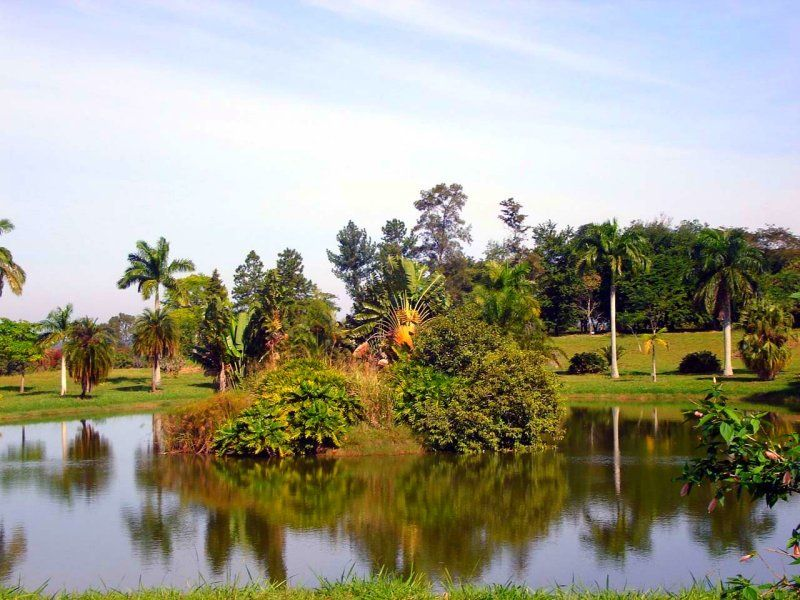
\includegraphics[width=16cm]{figura01}
\caption{Jardim Botânico da UFRuralRJ. Fonte: \url{http://commons.wikimedia.org/wiki/File:Jardim_Bot\%C3\%A2nico_UFRRJ.jpg}}
\label{fig:jardim}
\end{figure}

\blindtext[1]

\section{SEÇÃO}

\blindtext[2]

\subsection{Subseção}

\blindtext[2] %% Incluir capítulo 00
\artigotrue
\chapter{Título do Primeiro artigo}
\label{chap:chapter01}

\begin{chapterabstract}{brazilian}{Palavra-chave 1, Palavra-chave 2, Palavra-chave 3}
Este é o resumo do primeiro artigo da tese.
\end{chapterabstract}

\begin{chapterabstract}{english}{Key-word 1, Key-word 2, Key-word 3}
This is the abstract of the first article of the thesis.
\end{chapterabstract}

\formatchapter

\section{Introdução}

\blindtext[2]

\section{Material e métodos}

Este é um texto bem formatado, escrito em Seropédica, RJ. \blindtext[1]

Este é o código fote de uma função construída no ambiente R:

\begin{verbatim}
> soma <- function (a, b) {a + b}
> soma(2, 2)
[1] 4
\end{verbatim}

Está é uma matriz bem formatada:

\begin{equation}
  A_{m,n} =
 \begin{pmatrix}
  a_{1,1} & a_{1,2} & \cdots & a_{1,n} \\
  a_{2,1} & a_{2,2} & \cdots & a_{2,n} \\
  \vdots  & \vdots  & \ddots & \vdots  \\
  a_{m,1} & a_{m,2} & \cdots & a_{m,n}
 \end{pmatrix}
\end{equation}

\begin{subequations}\label{eq:maxwell}
E estas são as equações de Maxwell:
\begin{align}
        B'&=-\nabla \times E,\\
        E'&=\nabla \times B - 4\pi j,
\end{align}
\end{subequations}

\section{Resultados}

Aqui está mais um texto bem formatado. \blindtext[1]

Que tal fazer um link para a figura \autoref{fig:ocio}? E também citar o \citet{Feyerabend1977} com um link para a localização da referência bibliográfica?

\begin{figure}[!ht]
\centering
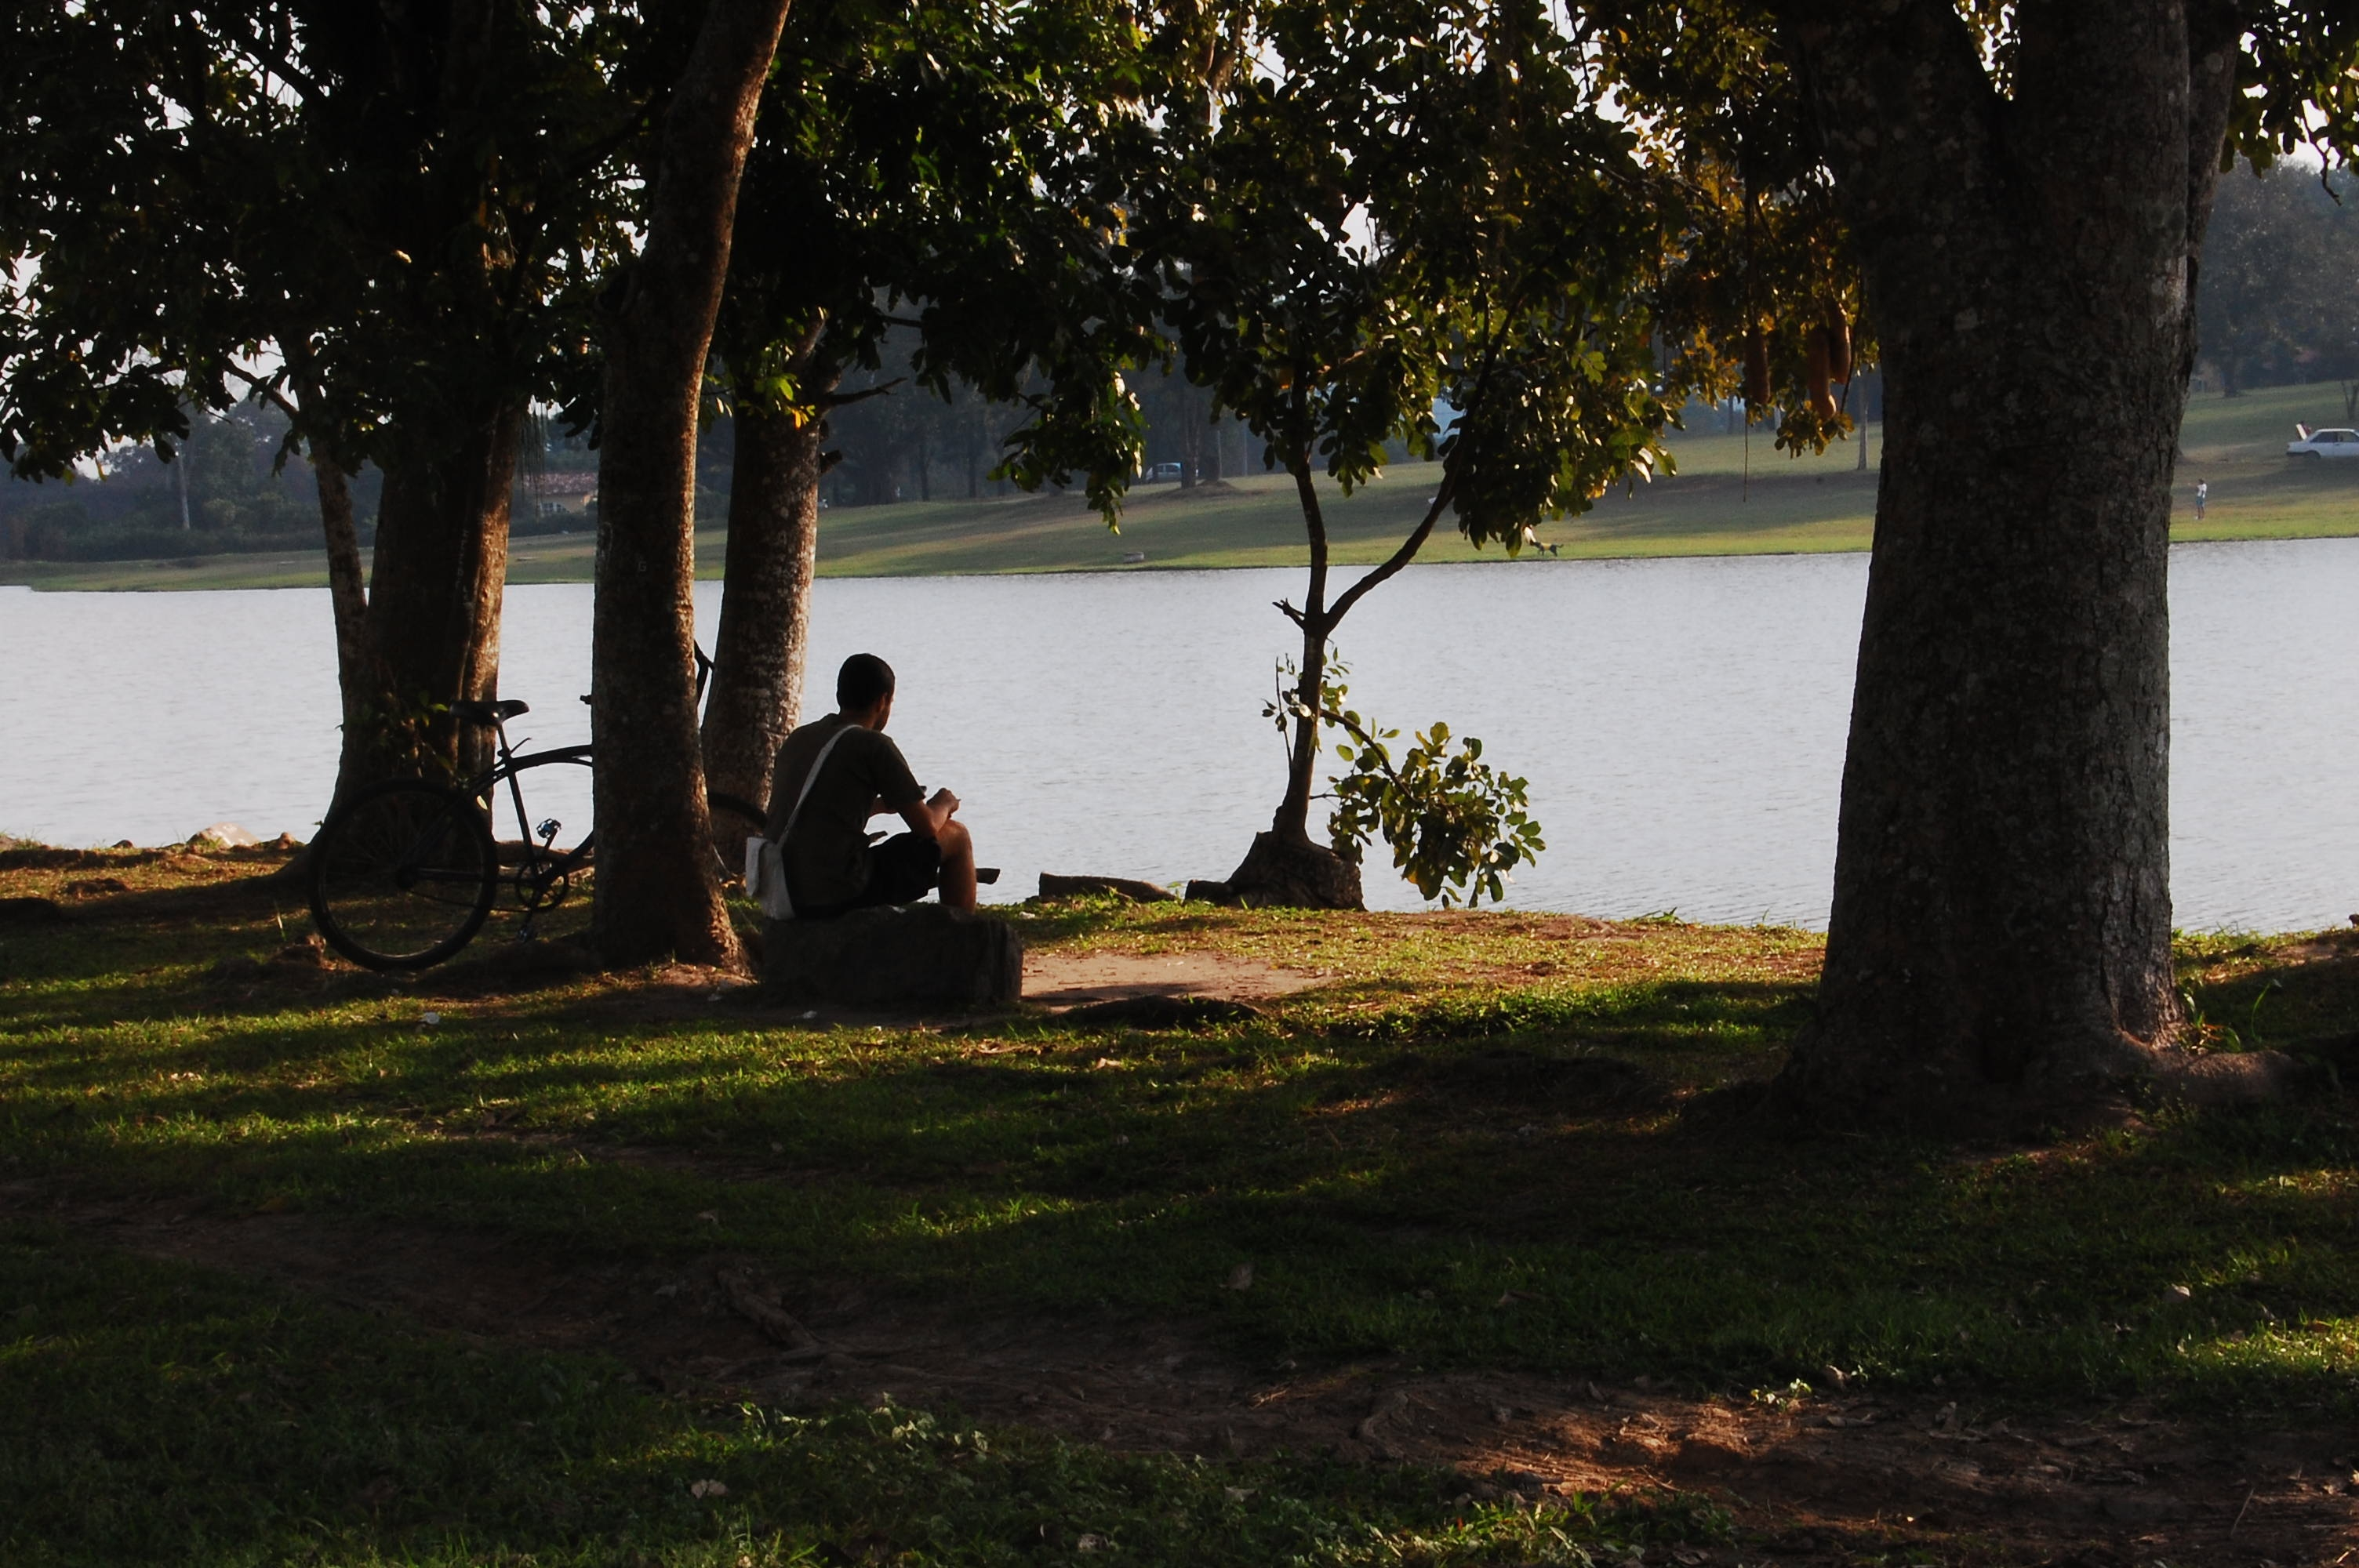
\includegraphics[width=16cm]{figura02}
\caption{\label{fig:ocio}O ócio criativo. Fonte: \url{http://r1.ufrrj.br/graduacao/img/acesso-2012/o-ocio-criativo.jpg}}
\end{figure}

\section{Discussão}

Aqui está o último texto muito bem formatado. \blindtext[2]

Que tal fazer um link para a equação \autoref{eq:maxwell}?

\section{Conclusões}

\begin{itemize}
  \item Está é uma conclusão importante.
  \item Está é outra conclusão importante.
  \item Está é uma conclusão menos importante.
\end{itemize}
 %% Incluir capítulo 01
\artigotrue
\chapter{TÍTULO DO SEGUNDO ARTIGO}
\chapternote{Este capítulo é baseado em um artigo que já foi publicado.}
\shorttitle{Segundo artigo}
\label{chap:chapter01}

\begin{chapterabstract}{brazilian}{Palavra-chave 1. Palavra-chave 2. Palavra-chave 3}
Este é o resumo do segundo artigo da tese. Reconheço que este artigo não é muito
diferente do anterior... Mas quem se importa?
\end{chapterabstract}

\begin{chapterabstract}{english}{Key-word 1. Key-word 2. Key-word 3}
This is the abstract of the second article of the thesis. I recognize that it is
not very different from the previous... But who cares?
\end{chapterabstract}

\formatchapter

\section{INTRODUÇÃO}

\blindtext[2]

\section{MATERIAL E MÉTODOS}

Este também é um texto bem formatado, escrito em Seropédica, RJ. \blindtext[1]

Este é o código fonte de uma função muito complexa construída no ambiente R:

\begin{verbatim}
> soma <- function (a, b) {a + b}
> soma(2, 2)
[1] 4
\end{verbatim}

Está é uma matriz bem formatada, diferente daquelas produzidas pelos editores de
texto tradicionais:

\begin{equation}
  A_{m,n} =
 \begin{pmatrix}
  a_{1,1} & a_{1,2} & \cdots & a_{1,n} \\
  a_{2,1} & a_{2,2} & \cdots & a_{2,n} \\
  \vdots  & \vdots  & \ddots & \vdots  \\
  a_{m,1} & a_{m,2} & \cdots & a_{m,n}
 \end{pmatrix}
\end{equation}

\begin{subequations}\label{eq:maxwell2}
E estas são as equações de Maxwell (sim, de Maxwell!):
\begin{align}
        B'&=-\nabla \times E,\\
        E'&=\nabla \times B - 4\pi j,
\end{align}
\end{subequations}

\section{RESULTADOS}

Para quem ainda não está cansado, aqui está mais um texto bem formatado. 
\blindtext[1]

Que tal fazer um link para a \autoref{fig:ocio2}? E também citar o 
\citeonline{Feyerabend1977} com um link para a localização da referência 
bibliográfica? Sim, isso já foi feito antes!

\begin{figure}[!ht]
\label{fig:ocio2}
\centering
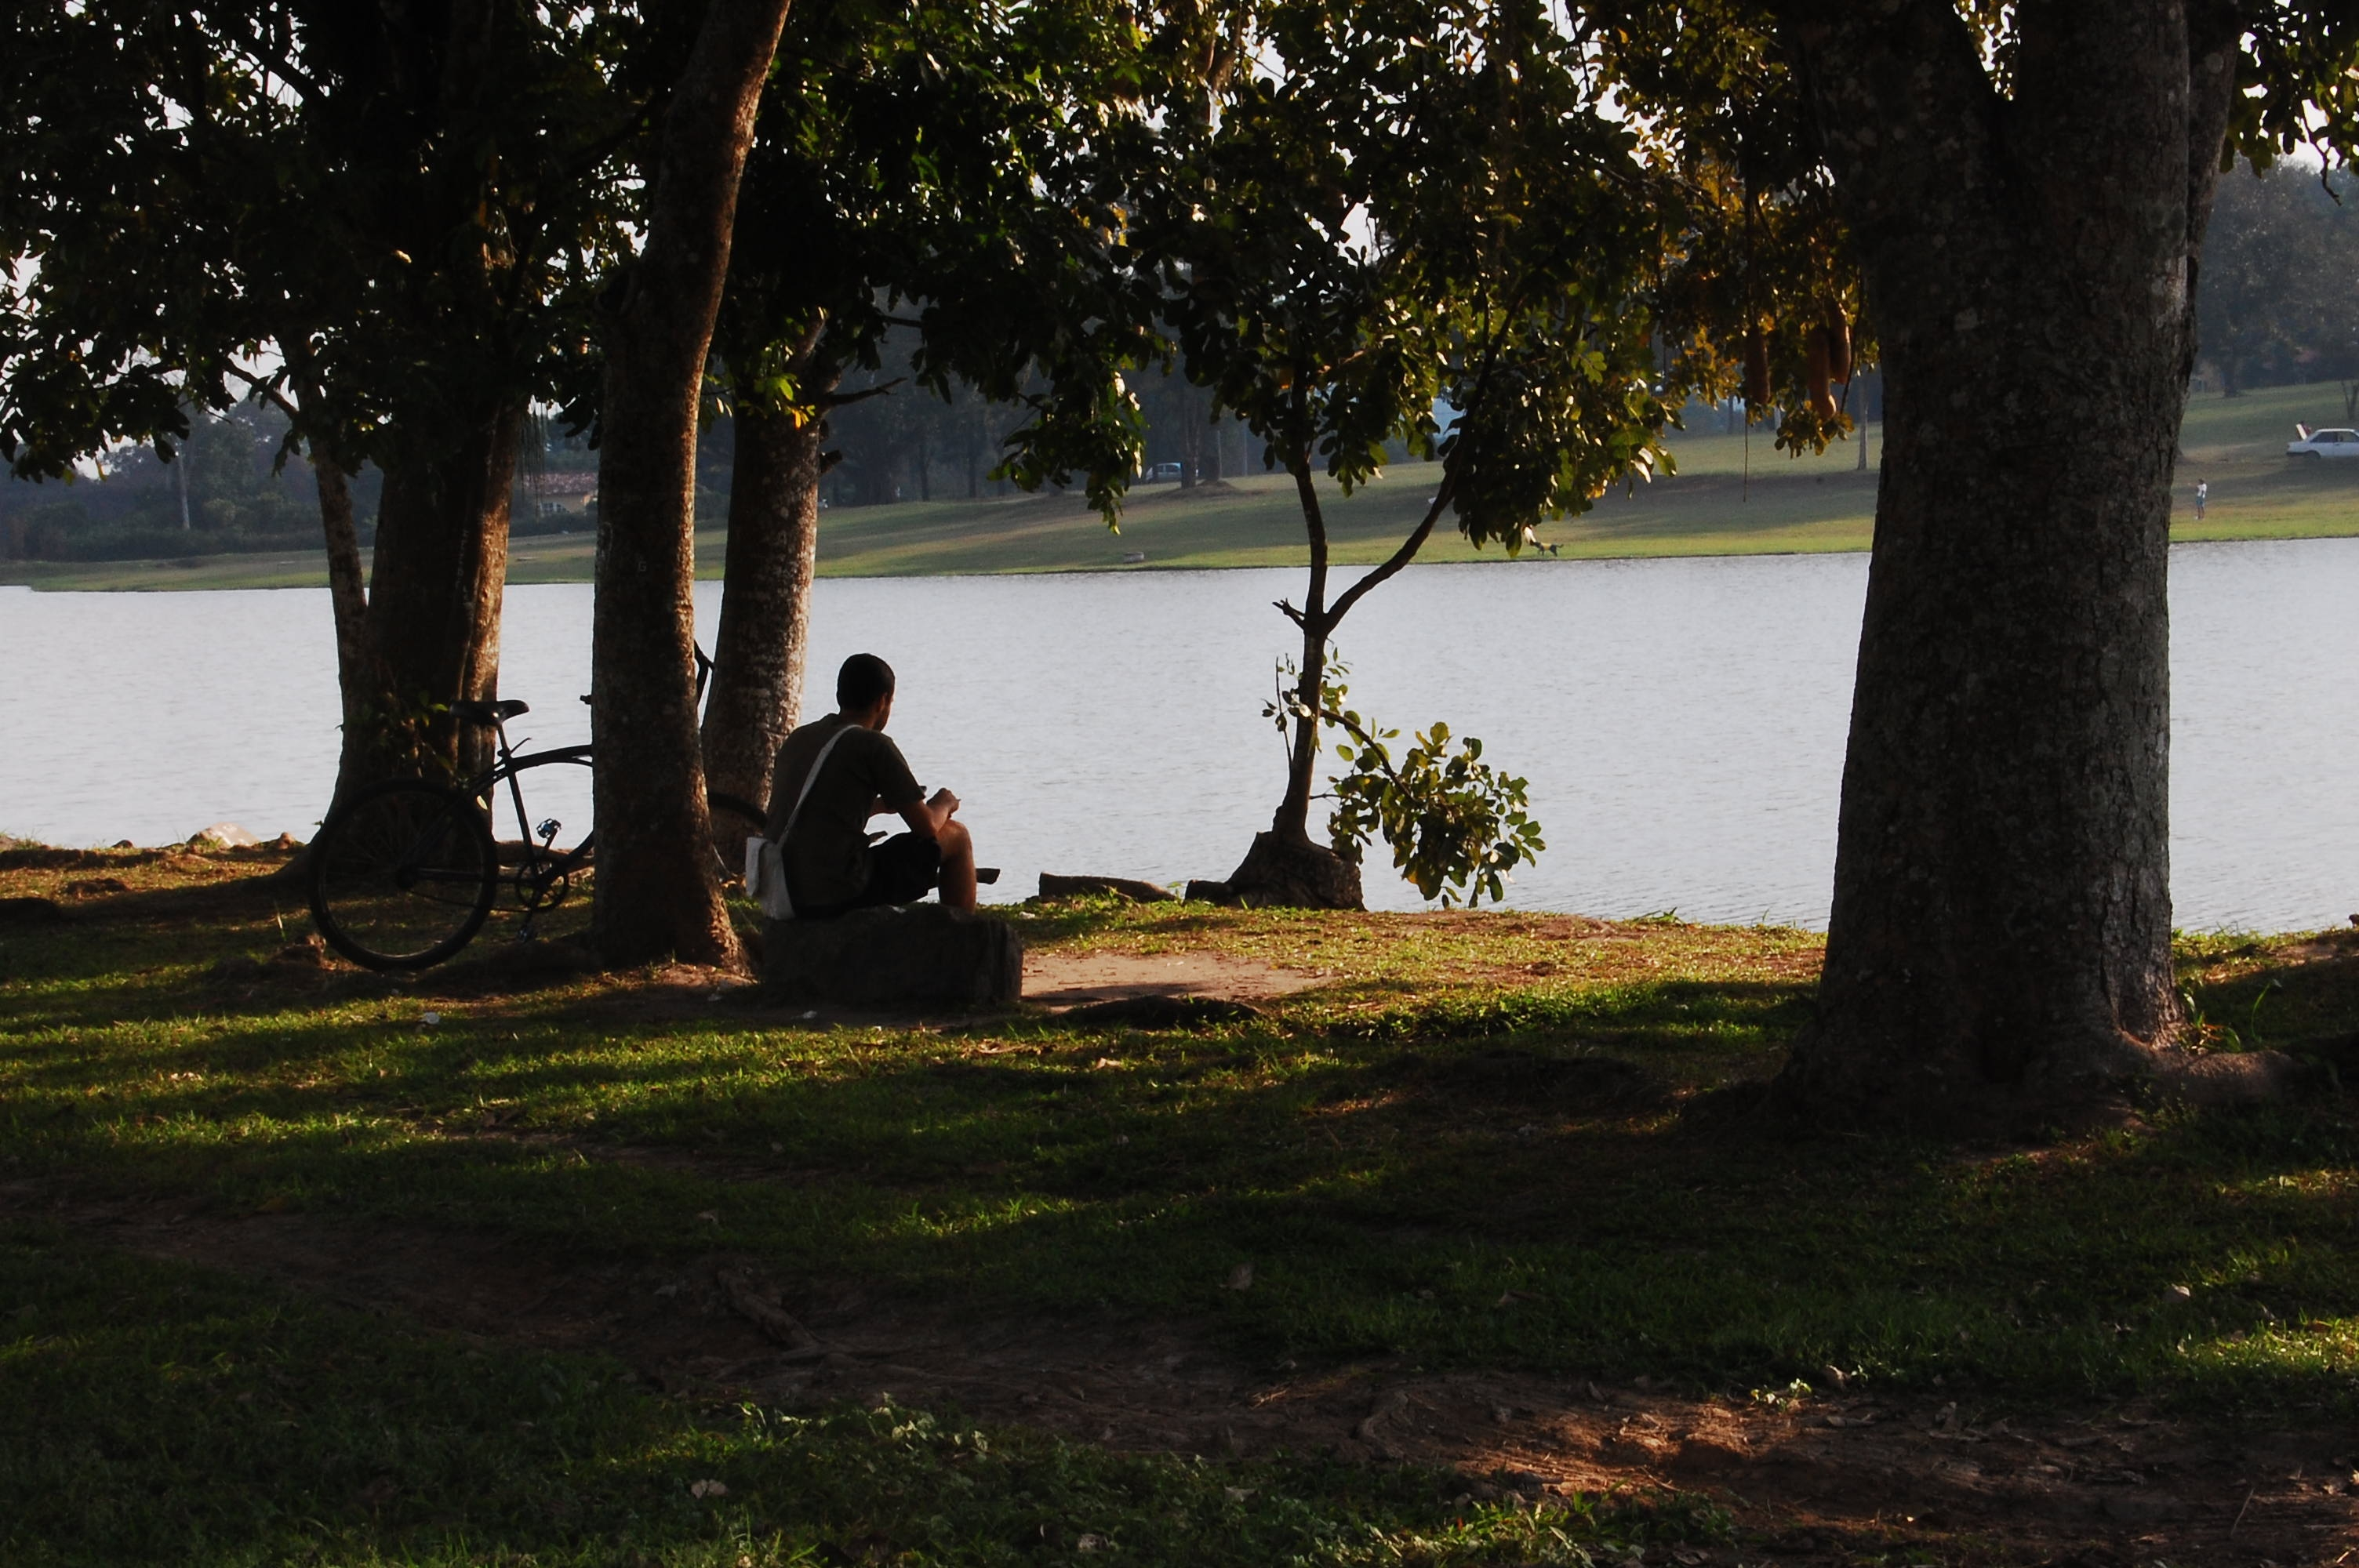
\includegraphics[width=16cm]{figura02}
\caption[O ócio criativo.]{O ócio criativo. Fonte: 
\url{http://r1.ufrrj.br/graduacao/img/acesso-2012/o-ocio-criativo.jpg}}
\end{figure}

\section{DISCUSSÃO}

Aqui está o último texto muito bem formatado. \blindtext[2]

Que tal fazer um link para a \autoref{eq:maxwell2}?

\section{CONCLUSÕES}

\begin{itemize}
  \item Está é uma conclusão importante.
  \item Está é outra conclusão importante.
  \item Está é uma conclusão menos importante.
\end{itemize}
 %% Incluir capítulo 02
\setlength{\baselineskip}{\baselineskip}

%%=============================================================================
%% Referências
%%=============================================================================

%% O arquivo 'biblio' com as referências bibliográficas deve estar no formato
%% BibTeX.
\bibliographystyle{abnt}
\bibliography{referencias-b/biblio}

%%=============================================================================
%% Apêndices e anexos
%% Se precisar usar alguma seção ou subseção dentro dos apêndices ou
%% anexos, utilizar o comando \tocless para não adicionar no Sumário
%% Exemplos: 
%% \tocless\section{Histórico}
%%=============================================================================

\appendix %% Apêndices
\artigofalse
\chapter{Primeiro apêndice}
\label{anex:apendiceA}

\tocless\section{Introdução}

\blindtext[2]

\tocless\section{Subseção}

\blindtext[2]
 %% Incluir apêndice A
%\include{capitulos-b/apendiceb} %% Incluir apêndice B

%\annex %% Anexos
%\include{capitulos-b/anexoa} %% Incluir anexo A
\end{document}